% LaTeX template for ECE2031
% Atneya Nair 
% 2020
% Some font and package installation may be required. MikTex or texlive-extra fonts is recommended. 

\documentclass[letterpaper,11pt]{article}
\usepackage[english]{babel}
\usepackage[margin=1in,footskip=0.25in]{geometry}
\usepackage[latin1]{inputenc}

% General figures and document formatting packages
\usepackage{graphicx}
\usepackage{titlesec}
\usepackage{float}
\usepackage[margin=10pt,font=small,labelfont=bf,
labelsep=period]{caption}

\usepackage[table,x11names]{xcolor} % tables
\usepackage{bold-extra} % bold fonts
\usepackage{listings} % code
\usepackage{varwidth} % overlines
\usepackage{csvsimple,booktabs} % tables from csv
\usepackage[title, titletoc]{appendix} % appendices
\usepackage{pdflscape} % landscape

\makeatletter
\g@addto@macro\@floatboxreset{\centering} % Center all floats 
\makeatother


% New page after section end
\newcommand{\sectionbreak}{\clearpage}

% Anchor floats
\floatplacement{table}{H}
\floatplacement{figure}{H}

% Table caption custom format
\DeclareCaptionFormat{centered}{%
  \begin{varwidth}{\linewidth}%
    \centering
    #1#2#3%
  \end{varwidth}%
}

% ECE 2031 caption format for tables and figures
\captionsetup[table]{labelfont={bf,sc}, format=centered, labelsep=newline, textfont={sc}}
\captionsetup[figure]{labelfont=bf, labelsep=period}

% Images and code are expected in a results subdirectory by default. Table importing from CSV is NOT.
% Code snippets default VHDL
\lstset{language=VHDL, basicstyle=\footnotesize, inputpath=./results/}
\graphicspath{{./results/}}

% Scale images greedily while maintaining aspect ratio. 
\setkeys{Gin}{width=\textwidth,height=\textheight,keepaspectratio}

% Convenience macro for figure insertion
\newcommand{\labfig}[2]{ %arg1 - fig path, arg2 - caption
\begin{figure}
\includegraphics{#1}
\caption{#2}
\end{figure}
}

%
\begin{document}

% Title setup
\title{Lab 1 Report}
\author{George P. Burdell \\
\emph{ECE 2031 L02}}          
\date{01 January 1970}
\maketitle
\thispagestyle{empty}
\tableofcontents
\newpage

\section{Unformatted Results}
% Beware of badbox with unformatted document scan images. Plentiful newpages is a good idea (or explicitly reduce width/height).
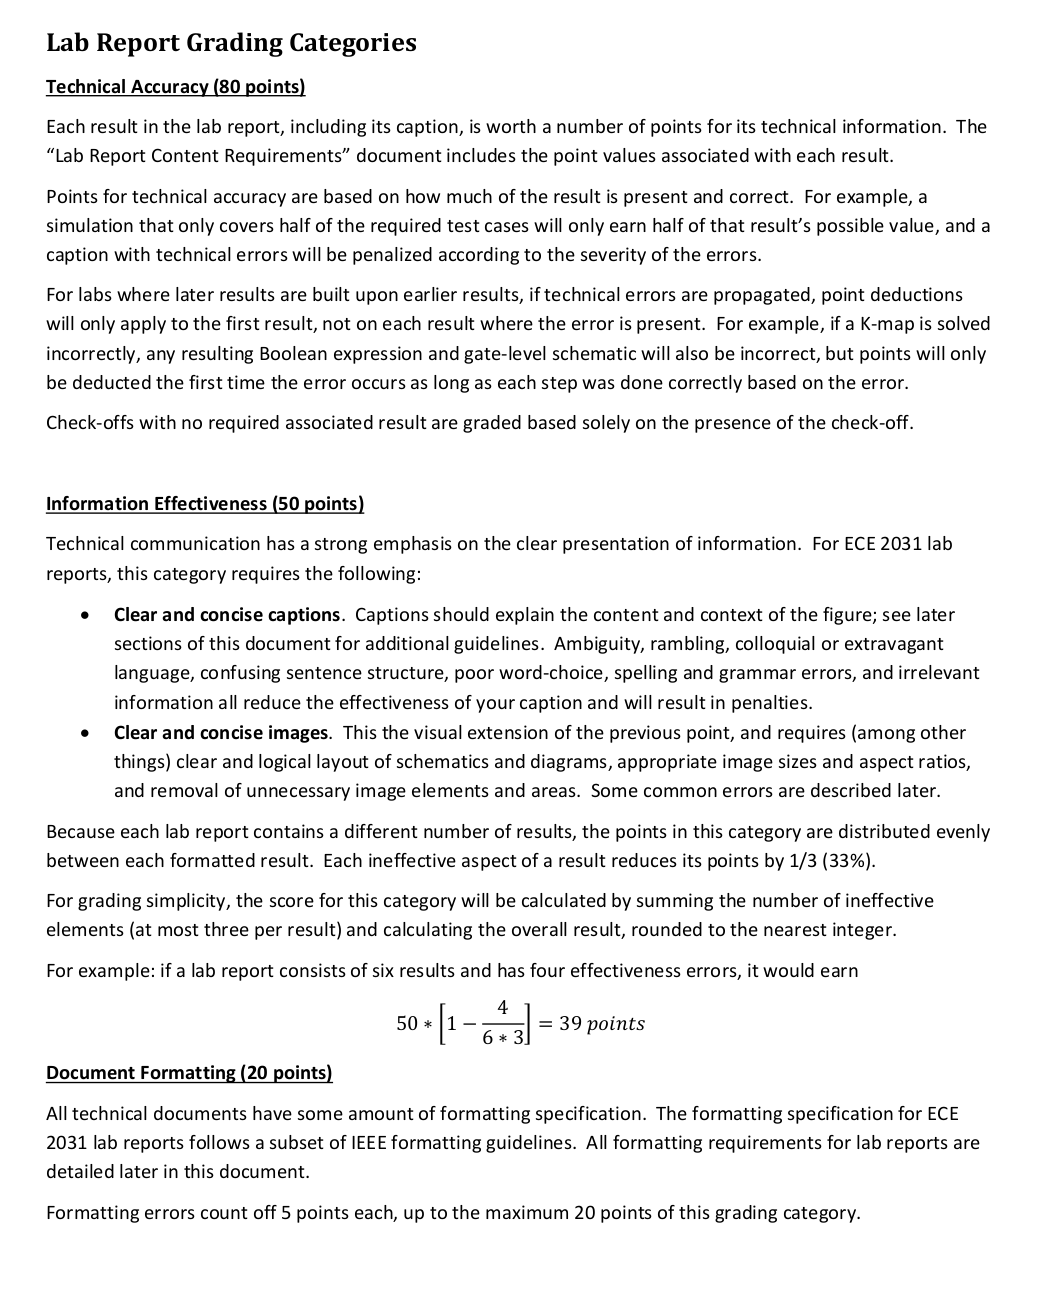
\includegraphics{unformatted.png}

\section{Results}


\begin{figure}
   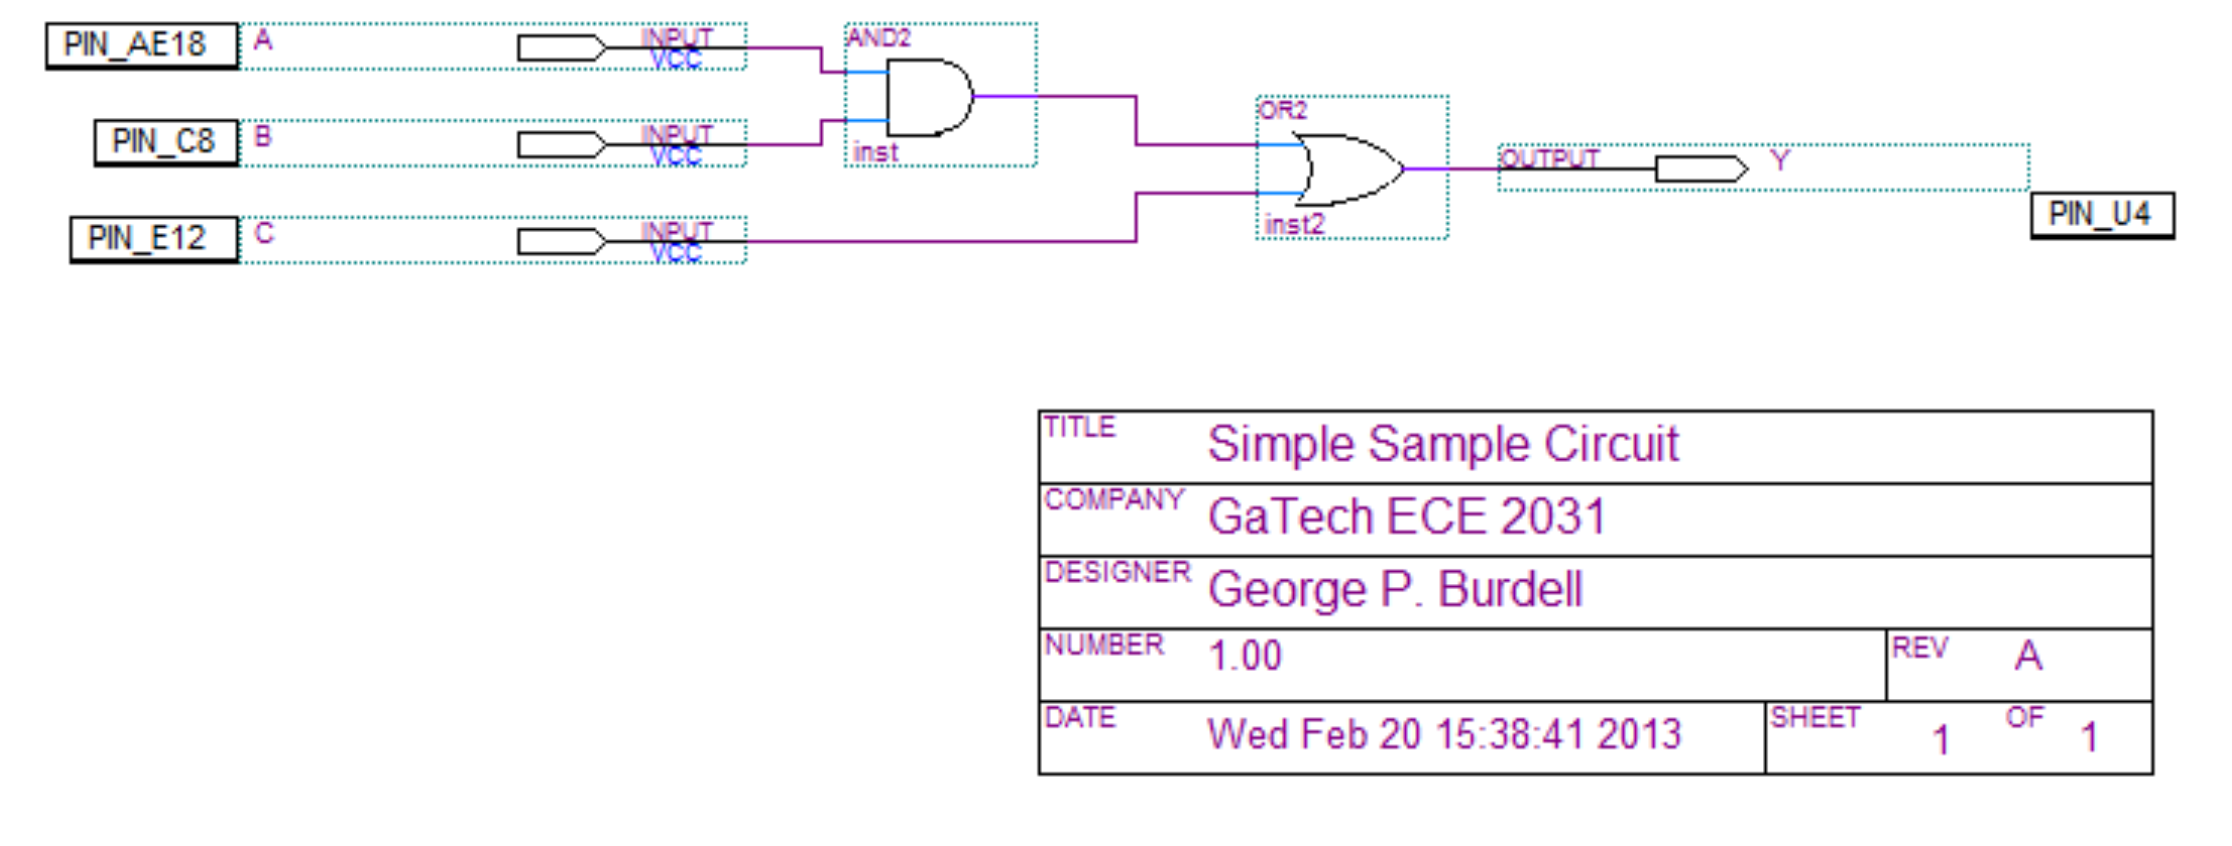
\includegraphics{simple_circuit.png} % from ./results/
      \caption{Schematic with FPGA pin assignments of circuit implementing $Y = AB + C$.} % One line caption, correctly formatted by setup
\end{figure}   



\labfig{complicated_circuit.png}{Circuit to light LED G8 when robot motors are enabled, and flash it at 10Hz when robot battery voltage is below minimum threshold.} % Using labfig macro to simplify figure insertion. This caption is also two lines 

\begin{landscape} % Correctly rotated landscape page (assuming single-sided printing). 
\begin{figure}
	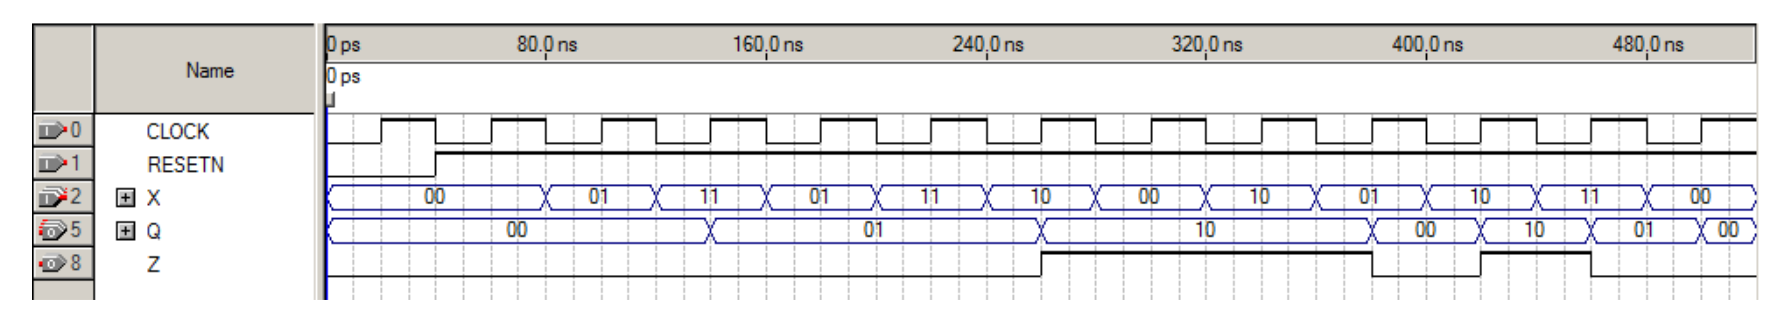
\includegraphics{landscape_figure.png}
	  \caption{Functional simulation waveform of state machine with three states, 2-bit input X, and 1-bit output Z. The input vector provides 100\% coverage of state transitions to prove correct behavior of the state machine, including assertion of Z in state '10 This figure should be properly rotated for both digital viewing and printing.}
\end{figure}
\end{landscape}

\begin{figure} % An explicitly inserted code fragment. See appendix for file import. Whitespace should be correctly pasted, as LaTeX follows whitespace verbatim.
% default listing language is VHDL for highlighting
	\begin{lstlisting} 
	-- ORGATE.VHD (VHDL)
	-- This code produces a negative-logic OR circuit
	-- George P. Burdell
	-- ECE2031 L01
	-- 01/31/2009
	
	LIBRARY IEEE;
	USE IEEE.STD_LOGIC_1164.all;


	ENTITY orgate IS
	PORT(
		PB1, PB2 : IN STD_LOGIC;
		LED : OUT STD_LOGIC);
	END orgate;

	ARCHITECTURE a OF orgate IS
	BEGIN
		LED <= NOT(NOT PB1 OR NOT PB2);
	END a;
	\end{lstlisting}
	\caption{VHDL code representing a three state, two input FSM satisfying the assigned state transitions, which outputs high only in state C.} % Captioning is treated like any other figure.
\end{figure}

\begin{table} % Explicitly inserted table, with correct caption (title) format from setup.
      \caption{Truth Table for $Y = \overline{ABC}$ With Highlights} % Below is a regular LaTeX array with some special formatting.
      % Replace values between ampersands and double slashes to change the data. Add a |c to add an additional column, as well as an additional & [value] in every row. The rest of the commands in the array are just visual flavor.
     $$ 
         \begin{array}{c|c}
            \hline
            \noalign{\smallskip}
                                ABC & Y \\
            \noalign{\smallskip}
            \hline
            \noalign{\smallskip}
								000 & 1 \\
								001 & 1 \\
								010 & 1 \\
								011 & 1 \\
			\hline
								100 & 1 \\
			\rowcolor{lightgray}101 & 1\\
								110 & 1 \\
			\rowcolor{lightgray}111 & 0 \\
            \noalign{\smallskip}
            \hline
         \end{array}
     $$ 
\end{table}

\begin{table}
      \caption{Truth Table for $Y = \overline{ABCD}$ From CSV} % We use the csvreader command to import a table from a standard CSV. Noteworthy parameters are explained below.
      \csvreader[
      	tabular=c|c,%Change tabular pre-amble i.e. additional 'c' for more centered columns, r/l for differently aligned, pipes/spaces to change the delimeter
      	before table=\rowcolors{2}{lightgray}{}, % Alternating row highlights set from xcolor before reading the csv
		table head=\toprule \bfseries $ABCD$ & \bfseries $Y$ \\ \midrule, % The first line of the table is defined here (labels and bounding lines), before reading from the CSV (but skipping the header row in the CSV).
		table foot=\bottomrule]  % Defines the final row of the table (after finishing reading the csv).
		{./results/nand.csv} % File location of csv to read from (no default directory/subdirectory, so a full relative path must be given)
    	{}
    	{\csvcoli & \csvcolii} % Add & \csvcol[column # in roman numeral] for additional columns
\end{table}



\begin{appendices} % Appendices for long code fragments 

% The following is an extremely messy command to format appendix titles on their own page (as well as the other specifications)
\titleformat{\section}[display]
{\filcenter\Large\sc}
{\clearpage~\vfill\appendixname~\thesection}
{5pt}
{}[\vfill\clearpage]

% Insert appendices below here.

\section{The first one} % Each begins with \section{[title]} within the appendices environment

\lstinputlisting{long_code.vhd} % Inserting VHDL code directly from a file (this should be greatly preferred). 

\section{The second one} % Again just to see how appendix formatting works

\lstinputlisting{long_code.vhd}

\end{appendices} % End of appendices environment

% If we ever needed a bibliography, we should make one below. 

%\begin{thebibliography}{}

%\end{thebibliography}

\end{document}
